% !TeX root = chapter-6-7-8.tex

\selectlanguage{hebrew}


\begin{comment}

\chapter{חקר פונקציות רציונליות}



\section{קיץ תשע"ז מועד ב}

\begin{center}
\selectlanguage{english}
\includegraphics[width=\textwidth]{summer-2017b-6}
\end{center}

\textbf{סעיף א}

$(1)$
תחום ההגדה הוא
$x\neq 2$
כי
$x=2$
מאפס את המכנה של שני גורמים.

$(2)$
כאשר 
$x\rightarrow \pm\infty$
שני גורמים שואפים לאפס, ולכן ה%
\asm{}
האופקית היא
$y=a$.

כאשר 
$x\rightarrow \pm 2$
שני גורמים שואפים לאינסוף, ולכן ה%
\asm{}
האנכית היא
$x=2$.

נבדוק את סימן הפונקציה השואפת לאינסוף. כאשר
$x\rightarrow 2$,
$\frac{1}{(x-2)^2}\gg\frac{2}{x-2}$
כך ש-%
$y\rightarrow+\infty$
גם מימין וגם משמאל.

$(3)$
\[
f'(x) = -\frac{2\cdot -1}{(x-2)^2} + \frac{-2}{(x-2)^3}=0\,.
\]
הפוקציה לא מוגדרת ב-% 
$x=2$,
כך שאפשר להכפיל את המשוואה ב-%
$(x-2)^3$.
נקבל
$2(x-2)=2$
ו-%
$x=3$.
נקודת הקיצון היא
$(3,a-1)$.

על ידי הכפלה ב-% 
$(x-2)$
וב-%
$(x-2)^2$
הנגזרת הראשונה היא:
\[
f'(x) = \frac{2(x-2)^2-2(x-2)}{(x-2)^4}=\frac{2x^2-10x+12)}{(x-2)^4}\,.
\]

\np

המכנה חיובי לכן הסימן של הנגזרת השנייה הוא סימן נגזרת המונה
$4x-10$.
ב-%
$x=3$,
הסימן חיובי והנקודת הקיצון היא מינימום.

דרך אחרת לבדוק אם מדובר במינימום או מקסימום היא באמצעות טבלת עליות וירידות:
\[
\begin{array}{c|c|c|c|c|c}
x & 0 & 2 & 2.5 & 3 & 4\\\hline
f'(x) & 0.75 & \times & -0.5& 0 & 0.25\\\hline
f(x) & \nearrow & \times & \searrow & a-1 & \nearrow
\end{array}
\]
הנקודה
$(3,a-1)$
היא מינימום.

$(4)$
ראו בסעיף הקודם.

\textbf{סעיף ב}

נתון שערכה של
$f(x)$
בנקודת המינימום הוא אפס.
$f(3)=a-1=0$
ו-%
$a=1$.

\textbf{סעיף ג}

לפי טבלת העליות והירידות, הפונקציה עולה עד ל%
\asm{}
האנכית, אח"כ יורדת לנקודת המינימום ואח"כ עולה.

\begin{center}
\selectlanguage{english}
\begin{tikzpicture}[scale=1]
\begin{axis}[
    xlabel = $x$,
    ylabel = {$f(x)$},
    axis lines=center,
    xtick={-2,...,7},
    ytick={-1,...,5},
    xmin = -2,
    xmax = 7,
    ymin = -1,
    ymax = 5,
    xticklabel style={
    anchor=north east,
    },
    yticklabel style={
    anchor=south east,
    },
    every axis y label/.style={at={(ticklabel cs:0.7)},rotate=90,anchor=west,},
    every axis x label/.style={at={(ticklabel cs:0.7)},anchor=north,},
]
\addplot [
    domain=-2:1.3, 
    samples=40, 
]
{1-(2/(x-2))+(1/(x-2)^2)};
\addplot [
    domain=2.3:7, 
    samples=40, 
]
{1-(2/(x-2))+(1/(x-2)^2)};
\draw[dashed,thick] ({axis cs:2,0}|-{rel axis cs:0,0}) -- ({axis cs:2,0}|-{rel axis cs:0,1});
\draw[dashed,thick] ({axis cs:-2,1}-|{rel axis cs:0,0}) -- ({axis cs:-2,1}-|{rel axis cs:7,0});
\fill (axis cs:3,0) circle(1.5pt);
\end{axis}
\end{tikzpicture}
\end{center}


\textbf{סעיף ד}
ה%
\asm{}
האופקית היא
$y=a=1$
ונקודת המינימום היא
$(3,a-1)=(3,0)$:
\begin{eqnarray*}
g(3)&=&|f(3)+k|=a=1\\
|0+k|&=&1\\
k&=&\pm 1\,.
\end{eqnarray*}


\section{קיץ תשע"ז מועד א}

\begin{center}
\selectlanguage{english}
\includegraphics[width=\textwidth]{summer-2017a-6}
\end{center}

\vspace{-5ex}

\textbf{סעיף א}


$(1)$
הפונקציה מוגדרת אם המכנה שונה מאפס ואם הביטוי בשורש גדול או שווה לאפס:
\begin{equationarray*}{rcl}
x^2-10x+24 &>& 0\\
(x-4)(x-6) &>& 0\,.
\end{equationarray*}
המכפלה חיובית רק אם שני הגורמים גדולים מאפס או שניהם קטנים מאפס. אבל אם 
$x>6$
אז 
$x>4$
ואם
$x<4$
אז 
$x<6$,
ולכן הפונקציה מוגדרת כאשר:
\[
x<4 \quad 
\textrm{\R{או}}
\quad x>6\,.
\]
$(2)$
$f(x)=0$
אם המכנה חיובי והמונה 
$x-5=0$.
אבל 
$5$
לא בתחום ההגדרה כך שאין נקודת חיתוך עם ציר ה-%
$x$.
חישוב נקודת החיתוך 
$(0,y)$
עם ציר ה-%
$y$:
\[
y=f(0)=\frac{0-5}{\sqrt{0^2-10\cdot 0 + 24}}=\frac{-5}{\sqrt{24}}\,.
\]
$(3)$
כאשר 
$x\rightarrow 6^{+}$
המונה שואף ל-%
$1$.
המכנה שורש חיובי שהולך וקטן, ולכן
$f(x)\rightarrow +\infty$.
$x=6$
היא
\asm{}
אנכית אחת. באופן דומה, כאשר
$x\rightarrow 4^{-}$,
$f(x)\rightarrow -\infty$,
ו-%
$x=4$
היא
\asm{}
אנכית שנייה.

כאשר 
$x\rightarrow +\infty$
המנה שואף ל-%
$+\infty$.
כאשר 
$x\rightarrow +\infty$,
במכנה
$x^2\gg -10x+24$,
וערכו מתקרב ל-%
$\sqrt{x^2}=x$
שגם הוא שואף ל-%
$+\infty$.
לכן
$y\rightarrow 1$
היא
\asm{}
אופקית אחת. באופן דומה, כאשר
$x\rightarrow -\infty$,
$y\rightarrow -1$
ו-%
$y=-1$
היא
\asm{}
אופקית שנייה.

\np

$(4)$
אי-אפשר פשוט להכין טבלה של עליות וירידות, כי אין אנו יודעים אם יש נקודות קיצון בתחום ההגדרה של הפונקציה. כצעד ראשון נבדוק את ערכו של
$f(x)'$.
לשם קיצור נסמן
$u=x^2-10x+24$.
הנגזרת היא:
\[
\frac{1\cdot \sqrt{u} - (x-5)\cdot \frac{1}{2} u^{-\frac{1}{2}} \cdot (2x-10)}{u}=\frac{u - (x-5)(x-5)}{u\sqrt{u}}\,.
\]
$u$
חיובי
\textbf{בתחום ההגדרה}
וגם
$\sqrt{u}$
חיובי, ולכן הסימן או נקודת האיפוס של הנגזרת תלוי רק במונה:
\[
u-(x-5)(x-5)=x^2-10x+24-x^2+10x-25=-1\,.
\]
בתחום ההגדרה, הנגזרת שלילית )ולא מתאפסת(, ולכן הפונקציה יורדת בכל תחום ההגדרה.

\vspace{1ex}
$(5)$

\vspace{-3ex}

\begin{center}
\selectlanguage{english}
\begin{tikzpicture}[scale=.9]
\begin{axis}[
    xlabel = $x$,
    ylabel = {$f(x)$},
    axis lines=center,
    xtick={-1,...,8},
    ytick={-3,...,3},
    xmin = -1,
    xmax = 8,
    ymin = -3,
    ymax = 3,
    xticklabel style={
    anchor=north east,
    },
    yticklabel style={
    anchor=south east,
    },
    every axis y label/.style={at={(ticklabel cs:0.7)},rotate=90,anchor=west,},
    every axis x label/.style={at={(ticklabel cs:0.7)},anchor=center,},
]
\addplot [
    domain=-1:3.9, 
    samples=40, 
]
{(x-5)/sqrt(x^2-10*x+24)};
\addplot [
    domain=6.1:8, 
    samples=40, 
]
{(x-5)/sqrt(x^2-10*x+24)};
\draw[dashed,thick] ({axis cs:4,-3}|-{rel axis cs:0,0}) -- ({axis cs:4,-3}|-{rel axis cs:0,6});
\draw[dashed,thick] ({axis cs:6,-3}|-{rel axis cs:0,0}) -- ({axis cs:6,-3}|-{rel axis cs:0,6});
\draw[dashed,thick] ({axis cs:-1,1}-|{rel axis cs:0,0}) -- ({axis cs:-1,1}-|{rel axis cs:9,0});
\draw[dashed,thick] ({axis cs:-1,-1}-|{rel axis cs:0,0}) -- ({axis cs:-1,-1}-|{rel axis cs:9,0});
\end{axis}
\end{tikzpicture}
\end{center}

\vspace{-3ex}

\textbf{סעיף ב}

$(1)$
פתרון אחד הוא לחשב את
$g(x),g(-x)$
ולהראות ש-%
$g(-x)=-g(x)$:

\vspace{-4ex}

\erh{11pt}
\begin{equationarray*}{rcl}
g(-x) &=& f(-x+5)=f(5-x)\\
&=& \frac{5-x-5}{\sqrt{(5-x)^2-10(5-x)+24}}\\
&=&\frac{-x}{\sqrt{25-10x+x^2-50+10x+24}}\\
&=&\frac{-x}{\sqrt{x^2-1}}\,,
\end{equationarray*}

\vspace{-7ex}

\erh{11pt}
\begin{equationarray*}{rcl}
g(x) &=& f(x+5)\\
&=& \frac{x+5-5}{\sqrt{(x+5)^2-10(x+5)+24}}\\
&=&\frac{x}{\sqrt{x^2+10x+25-10x-50+24}}\\
&=&\frac{x}{\sqrt{x^2-1}}\,.
\end{equationarray*}

\vspace{-3ex}

\np

פתרון מעט יותר מסובך הוא להראות
$g(-x)=-g(x)$
בצורה ישירה:
\erh{12pt}
\begin{equationarray*}{rcl}
g(-x) &=& f(-x+5)=f(5-x)\\
&=& \frac{5-x-5}{\sqrt{(5-x)^2-10(5-x)+24}}\\
&=&\frac{-x}{\sqrt{25-10x+x^2-50+10x+24}}\\
&=&\frac{-x}{\sqrt{x^2+10x+25-10x-50+24}}\\
&=&\frac{-((x+5)-5)}{\sqrt{(x+5)^2-10(x+5)+24}}\\
&=&-g(x)\,.
\end{equationarray*}

\vspace{-3ex}

$(2)$
הגרף הוא אותו גרף מוזז שמאלה חמש יחידות:

\begin{center}
\selectlanguage{english}
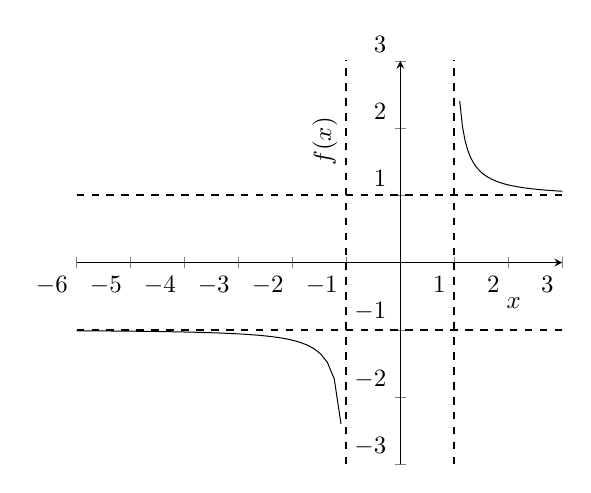
\begin{tikzpicture}[scale=.9]
\begin{axis}[
    xlabel = $x$,
    ylabel = {$f(x)$},
    axis lines=center,
    xtick={-6,...,3},
    ytick={-3,...,3},
    xmin = -6,
    xmax = 3,
    ymin = -3,
    ymax = 3,
    xticklabel style={
    anchor=north east,
    },
    yticklabel style={
    anchor=south east,
    },
    every axis y label/.style={at={(ticklabel cs:0.8)},rotate=90,anchor=south,},
    every axis x label/.style={at={(ticklabel cs:0.9)},anchor=center,},
]
\addplot [
    domain=-6:-1.1, 
    samples=40, 
]
{x/sqrt((x+5)^2-10*(x+5)+24)};
\addplot [
    domain=1.1:3, 
    samples=40, 
]
{x/sqrt((x+5)^2-10*(x+5)+24)};
\draw[dashed,thick] ({axis cs:-1,-3}|-{rel axis cs:0,0}) -- ({axis cs:-1,-3}|-{rel axis cs:0,6});
\draw[dashed,thick] ({axis cs:1,-3}|-{rel axis cs:0,0}) -- ({axis cs:1,-3}|-{rel axis cs:0,6});
\draw[dashed,thick] ({axis cs:-6,1}-|{rel axis cs:0,0}) -- ({axis cs:-6,1}-|{rel axis cs:9,0});
\draw[dashed,thick] ({axis cs:-6,-1}-|{rel axis cs:0,0}) -- ({axis cs:-6,-1}-|{rel axis cs:9,0});
\end{axis}
\end{tikzpicture}
\end{center}

\textbf{סעיף ג}

נתון ש-%
$1<a<b$,
וכפי שניתן לראות מהגרף,
$a,b$
הם בתחום ההגדרה של 
$g$.
נחשב:
\[
\int_a^b g(x) dx = \int_a^b f(x+5) dx = \int_{a+5}^{b+5} f(x) dx\,.
\]

\end{comment}

\section{קיץ תשע"ז מועד ב}

\begin{center}
\selectlanguage{english}
\includegraphics[width=\textwidth]{summer-2015b-6}
\end{center}

\textbf{סעיף א}

$(1)$
ערך הוא מחוץ לתחום ההגדרה כאשר הוא מאפס את המכנה. 
$\sin 0=0$, $\cos \frac{\pi}{2}= \cos -\frac{\pi}{2}=0$ 
ותחום ההגדרה הוא:
\[
-\frac{\pi}{2} < x < 0,\quad 0 < x < \frac{\pi}{2}\,.
\]

$(2)$
הפונקציה סינוס היא אי-זוגית והפונקציה קוסינוס היא זוגית. המכפלה שלהן היא אי-זוגיות.

$(3)$
\[
((\sin x \cos x)^{-1})'= -1\cdot (\sin x \cos x)^{-2}(\sin x\cos x)'\,.
\]
בתחום ההגדרה המכנה חיובי, כך שנאשר רק לבדוק אם המונה יכול להתאפס.
\[
-(\sin x\cos x)'=-(\cos^2 x-\sin^2 x)=(\sin^2 x-\cos^2 x)=0\,.
\]
נקודות הקיצון הן בערכים שיש להם ערך מוחלט של סינוס שווה לערך מוחלט של קוסינוס, שהם כפולות של 
$\frac{\pi}{4}$.
בתחום ההגדרה:
\[
x=\pm\frac{\pi}{4},\quad y=\frac{2\cdot 2}{\pm\sqrt{2}\cdot\sqrt{2}}=\pm 2\,.
\]

\np

המכנה של הנגזרת הראשונה הוא 
$(\sin x \cos x)^2$,
ערך חיובי בתחום ההגדרה, ולכן, סימן הנגזרת השנייה הוא כסימן הנגזרת של המונה.
\[
(\sin^2 x-\cos^2 x)'=2\sin x \cos x -2 \cos x (-\sin x)=4\sin x\cos x\,.
\]
עבור
$x=\frac{\pi}{4}$,
$4\sin x\cos x=2<0$
והנקודה היא מינימום.

עבור
$x=-\frac{\pi}{4}$,
$4\sin x\cos x=-2<0$
והנקודה היא מקסימום.

$(4)$
\begin{center}
\selectlanguage{english}
\begin{tikzpicture}[scale=.9]
\begin{axis}[
    trig format plots=rad,
    axis lines=center,
    xmin=-1.57,
    xmax=1.57,
    xtick={-1.57,-.785,0,.785,1.57},
    xticklabels={$-\frac{\pi}{2}$,$-\frac{\pi}{4}$,$0$,
                 $\frac{\pi}{4}$,$\frac{\pi}{2}$},
    ymin = -4,
    ymax = 4,
    ytick={-2,2},
    yticklabels={$-2$,$2$},
    xticklabel style={anchor=north east,},
]
\addplot [
    domain=-1.55:-.05, 
    samples=40, 
]
{1/(sin(x)*cos(x))};
\addplot [
    domain=.05:1.55, 
    samples=40, 
]
{1/(sin(x)*cos(x))};
\draw[dashed,thick] ({axis cs:-1.57,-4}|-{rel axis cs:0,0}) -- ({axis cs:-1.57,-4}|-{rel axis cs:0,3.14});
\draw[dashed,thick] ({axis cs:1.57,-4}|-{rel axis cs:0,0}) -- ({axis cs:1.57,-4}|-{rel axis cs:0,3.14});
\fill (axis cs:.785,2) circle(1.5pt);
\fill (axis cs:-.785,-2) circle(1.5pt);
\end{axis}
\end{tikzpicture}
\end{center}

\textbf{סעיף ב}

$(1)$
למשוואה פתרון אחד אם הגרף משיק לציר ה-%
$x$
או חותך את הציר במקום אחד בלבד. מצב זה מתקבל כאשר 
$a=\pm 2$
שמעלה או מוריד את הגרף בשתי יחידות.

\begin{center}
\selectlanguage{english}
\begin{tikzpicture}[scale=.9]
\begin{axis}[
    trig format plots=rad,
    axis lines=center,
    xmin=-1.57,
    xmax=1.57,
    xtick={-1.57,-.785,0,.785,1.57},
    xticklabels={$-\frac{\pi}{2}$,$-\frac{\pi}{4}$,$0$,
                 $\frac{\pi}{4}$,$\frac{\pi}{2}$},
    ymin = -6,
    ymax = 6,
    ytick={-2,2},
    yticklabels={$-2$,$2$},
    xticklabel style={anchor=north east,},
]
\addplot [
    domain=-1.55:-.05, 
    samples=40, 
]
{(1/(sin(x)*cos(x)))-2};
\addplot [
    domain=.05:1.55, 
    samples=40, 
]
{(1/(sin(x)*cos(x)))-2};
\draw[dashed,thick] ({axis cs:-1.57,-4}|-{rel axis cs:0,0}) -- ({axis cs:-1.57,-4}|-{rel axis cs:0,3.14});
\draw[dashed,thick] ({axis cs:1.57,-4}|-{rel axis cs:0,0}) -- ({axis cs:1.57,-4}|-{rel axis cs:0,3.14});
\fill (axis cs:.785,0) circle(1.5pt);
\fill (axis cs:-.785,-4) circle(1.5pt);
\end{axis}
\end{tikzpicture}
\hspace{2em}
\begin{tikzpicture}[scale=.9]
\begin{axis}[
    trig format plots=rad,
    axis lines=center,
    xmin=-1.57,
    xmax=1.57,
    xtick={-1.57,-.785,0,.785,1.57},
    xticklabels={$-\frac{\pi}{2}$,$-\frac{\pi}{4}$,$0$,
                 $\frac{\pi}{4}$,$\frac{\pi}{2}$},
    ymin = -6,
    ymax = 6,
    ytick={-2,2},
    yticklabels={$-2$,$2$},
    xticklabel style={anchor=north east,},
]
\addplot [
    domain=-1.55:-.05, 
    samples=40, 
]
{(1/(sin(x)*cos(x)))+2};
\addplot [
    domain=.05:1.55, 
    samples=40, 
]
{(1/(sin(x)*cos(x)))+2};
\draw[dashed,thick] ({axis cs:-1.57,-4}|-{rel axis cs:0,0}) -- ({axis cs:-1.57,-4}|-{rel axis cs:0,3.14});
\draw[dashed,thick] ({axis cs:1.57,-4}|-{rel axis cs:0,0}) -- ({axis cs:1.57,-4}|-{rel axis cs:0,3.14});
\fill (axis cs:.785,4) circle(1.5pt);
\fill (axis cs:-.785,0) circle(1.5pt);
\end{axis}
\end{tikzpicture}

\end{center}


\begin{comment}

\np

\section{המלצות}

\begin{itemize}
\item
אי-אפשר להכין טבלה של עליות וירידות עד שלא מחשבים את תחום ההגדרה וכל נקודות הקיצון של הפנוקציה, כי רק ביניהם אפשר לסמוך על זה שאין שינוי בכיוון הפונקציה.

\end{itemize}

\end{comment}


\selectlanguage{english}

